\chapter{Design and Evaluation of Techniques for HPC platforms with SDN-capable Interconnects} 
In this work, I explore the integration of software-defined networking (SDN) into high performance computing (HPC) systems, with a focus on adapting SDN mechanisms to the distinct communication characteristics of HPC applications.

This investigation is motivated by the widespread success of SDN in domains such as data centers, campus networks, and wide-area networks, where it has demonstrated significant improvements in traffic management and network resource optimization through features like logically centralized control, per-flow management, and programmability. Prior studies, including those by Kreutz et al.\ and He et al., have shown how SDN can optimize Internet and data-parallel workloads through dynamic reconfiguration and intelligent traffic steering.

These efforts, while impactful, primarily target Internet and data-parallel applications characterized by coarse-grained, irregular traffic patterns, and fall short in addressing the repetitive communication phases inherent to HPC workloads. As a result, conventional SDN techniques, when applied to HPC systems, often incur prohibitive overheads due to their inability to react efficiently to short-duration, phase-driven communication behavior. Consequently, SDN remains underutilized in HPC environments, highlighting the need for novel techniques that can effectively leverage the static and predictable nature of many HPC communication patterns.

To address the challenges of applying SDN in HPC environments, I introduce techniques that leverage the communication behavior exhibited by HPC applications, specifically focusing on flow identification and communication phase identification. A large number of HPC applications simulate physical processes over numerous time steps, with each time step performing similar tasks that alternate between computation and communication phases. These communication phases often repeat and, in many applications, occur at durations in the order of subseconds or even submilliseconds, making conventional SDN techniques unsuitable due to the overheads incurred when reacting to such fine-grain behavior. However, because these communication patterns are often static and either known to application developers or can be analyzed statically or dynamically, they present an opportunity for SDN systems to optimize their operation. I propose flow identification to accurately classify application flows, with particular focus on elephant flows---those that carry large amounts of data and typically dominate the communication time. Identifying and efficiently scheduling these elephant flows helps address the problem of unbalanced network traffic in HPC applications. Additionally, I distinguish between static and dynamic communications, using application-provided hints through an API to guide flow classification for static patterns, and employing a machine learning--based approach to support flow identification in dynamic cases.

To evaluate the effectiveness of the proposed techniques, I conduct extensive simulation experiments using the TraceR-CODES parallel discrete-event simulator on a 3-level Fat-tree topology. These simulations include both static and dynamic communication benchmarks to assess the applicability of the approach across a range of HPC workloads. For static applications such as Stencil4d, which involve near-neighbor communication patterns, the techniques I present result in notable performance improvements. For dynamic applications such as Milc, where different communication patterns are exercised across iterations, the integration of application-level hints and machine learning--based flow identification demonstrates consistent advantages over existing SDN schemes. The evaluation across all three Fat-tree topologies confirms that incorporating communication-aware strategies into the SDN framework improves performance for both predictable and unpredictable communication behaviors. These results highlight the importance of aligning SDN control mechanisms with the underlying structure of HPC communication, particularly in systems where efficient flow management directly influences application scalability.

In summary, I contribute to the ongoing effort of adapting software-defined networking to the unique requirements of high performance computing systems by exploiting the repetitive and predictable communication behaviors of HPC applications. By bridging the gap between general-purpose SDN architectures and the fine-grained, phase-driven communication patterns common in scientific computing, I offer a communication-aware control strategy that enhances flow management in HPC networks. These contributions demonstrate that combining static flow information with dynamic identification mechanisms enables SDN to support both regular and irregular communication patterns, ultimately improving performance in realistic HPC workloads and guiding future directions in adaptive network control.


\section{Flow Classification in HPC Applications}
Data centers and HPC systems differ significantly in terms of their traffic characteristics. While the majority of traffic in a data center is small-scale, unpredictable, and not localized to any one level of the switch, traffic in an HPC application is primarily near-neighbor traffic, and may not be modest flows. Traditional flow identification methods may not be effective
in HPC environments. To effectively support SDN in the HPC environment,
novel techniques that take HPC communication characteristics into
consideration are proposed. Since a significant portion of
communications in HPC applications are static, we propose to have an API for
applications to provide flow information to the network directly. For
dynamic communications, we develop a machine learning based approach for
flow identification.

Figure~\ref{fig:flow_schemes} shows the high-level view of the proposed
flow classification systems. The flow classification techniques can
be classified into two types, those {\em with no extra user information} and
those {\em with user information}. The components below SDN API are similar to
traditional SDN systems. The flow classifier may take traffic statistics from
SDN switches and performs flow classification with no extra user information.
The classifier also allows HPC applications (SDN user) to directly give
hints about their communications to the network through an API
(similar to the intent-based API \cite{Coflow2012}), and classifies
such flows based on user information.

\begin{figure}[h]
\centering
    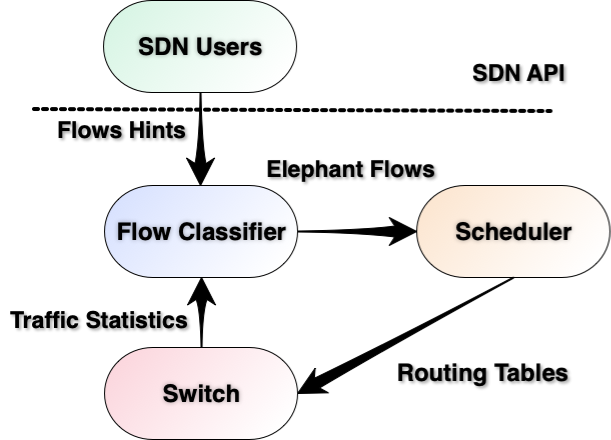
\includegraphics[width=0.8\columnwidth]{figs/Fig3.png}
\caption{High-level view of our flow classification schemes}
  \label{fig:flow_schemes}
\end{figure}

\subsection{Flow identification without user input}


\vspace{0.08in}
\noindent{\bf Threshold-based scheme}:
Existing flow classification methods including end host-based
management~\cite{xu2015identifying},
packet sampling~\cite{suh2014opensample}~\cite{afek2015sampling},
and polling per-flow statistics~\cite{yang2020flow}, do not assume
the type of applications. In this work, we compare our proposed techniques with
the classic elephant flow detection using a polling-based approach,
which is based on Hedera's architecture \cite{al2010hedera}.
Hedera's control loop comprises
three main components: flow detection, channel calculation, and channel
placement. Initially, significant 
flows are detected at the edge switches, and appropriate channels for these 
large flows are calculated using placement algorithms, taking into account 
their natural demand. These pathways are then placed on the switches.
%Hedera's architecture supports all common multi-rooted tree topologies.

Due to the overhead concerns, there is a limit how fast the flow statistics
are gathered, and path calculation and installations are performed, which is typically
in the order of seconds \cite{al2010hedera}.
However, in the HPC environment, depending
on applications, the time for each iteration may be much less than a second.
Hence, these existing flow classification schemes will miss many iterations
of application execution and not effective for such HPC applications.
To perform flow classification effectively for HPC systems, we develop
a machine learning based approach using deep neural network (DNN)
for flow classification.

\vspace{0.08in}
\noindent{\bf Deep learning-based scheme}:
As mentioned earlier, communications in HPC applications exhibits phase
behavior. If such behavior can be characterized and learned, we can classify
the flows quicker (after a small number of phases).
The information to differentiate between large elephant flows from
small mice flows is fundamentally captured by the time sequence of packets.
By training a Deep Neural Network (DNN) model using the time sequence of
packets from HPC workloads, the DNN model is able to recognize the
patterns of elephant flows in HPC applications. We note that the patterns
learned by the DNN model goes beyond simple statistics like
the existing threshold-based scheme: the model can also reflect more
sophisticated patterns such as the phased behavior. 


\vspace{0.08in}
\noindent{\em Model architecture}:
Our DNN model consists of an input layer of size 300 to accept the input data
which consists of data sent across various intervals of time and a single dense layer with
one output neuron, which uses the sigmoid activation function to classify the flows as elephants or mice.
The sigmoid function is commonly used for binary classification tasks
as it outputs a value between 0 and 1, which can be 
interpreted as the probability of the input belonging to the positive class. 
The model uses the Nadam optimizer with a learning rate of 0.01. Nadam is an 
extension of the popular Adam optimizer that incorporates Nesterov momentum, 
which helps to accelerate convergence. The model is compiled with binary 
cross-entropy loss, which is a standard loss function used for binary 
classification tasks.

\vspace{0.08in}
\noindent{\em Data collection and model training}:
We utilized the TraceR-CODES simulator to execute representative HPC 
workloads, namely Random-Permutation, Shift-256, Stencil3d, Stencil4d, Milc, Nekbone, Subcom3d-a2a, Kripke ~\cite{kripke}, Laghos, 
SW4lite ~\cite{sjogreen2018sw4}, and AMG ~\cite{amg}, 
for ranks ranging from 32 to 512. More detailed description of these
workloads is given in Section~\ref{sec:exp}.
Flow statistics were collected every 0.3 
seconds or 1\%
of the simulation to maintain minimal granularity. The flow data 
was gathered independently for each rank and merged to train the DNN 
model. For training purposes, the flows are marked as elephant or
mouse flows with a cut-off of $3 * 10^8$ bytes of data transfer in 90 seconds: 
Elephant flows were those transferring more than 300 MB of data in
90 seconds, while mouse flows were 
those transferring less. We employed a min-max scalar to scale the flow data 
before inputting it into the dense neural network layer for forecasting. The 
developed model was used offline to forecast network flows of elephants
or mice for systems running a combination of the aforementioned
applications.

During training, the model is trained on the input data and
corresponding binary labels. The total data is split as follows 20\%
of the training data is used for validation, while the remaining 80\% is 
used for training. Table~\ref{tab:model_acc} shows the model prediction
accuracy: the model prediction accuracy is very high for the data. 
We first trained the model on the applications which we are going to use for our simulations and 
see how it performed which are Random-Permutation, Shift-256, Stencil3d, Stencil4d, Milc, Nekbone and later on we added Subcom3d-a2a, Kripke , Laghos, SW4lite, and AMG for training to see if the model is able to handle the new data, along with the existing data and still provide a accurate prediction. We do this to make sure that our model is capable of getting  updated with new traffic as an when it comes. 

\begin{comment}
\paragraph{Model Offline Prediction}				
We conducted a study on three workloads generated by randomly selecting 
applications from Stencil4d, Subcom3d-a2a, Kripke, Laghos, AMG,
and SW4lite for  
ranks 32, 64, 128, 256, and 512. The TraceR-CODES simulator was used to 
simulate the corresponding workloads, and the flow data was collected.
The network flows that we gathered 
for the workload were predicted using the model. 

To validate the model's ability to forecast elephants and mice for any 
applications, we tested the model on unknown data. The model was employed to 
forecast the network flows of the application while it was operated 
individually and as a workload, and in each case, the model accurately 
predicted the flows by more than 95\%. The data used for making the 
predictions are presented in the table below.

Overall, our study demonstrates the effectiveness of the proposed neural 
network model for accurately predicting network flows of elephant and mice for 
various applications, which can assist in improving the performance of HPC 
systems.
%
\end{comment}

\begin{table}[h]
  \centering
  \caption{Accuracy of predicting elephants and mice flows by the DNN model for averaged across 32, 64, 128, 256 and 512 ranks}
    \label{tab:model_acc}
    \begin{tabular}{lr} \toprule
\multirow{1}{*}{Applications} & Accuracy \\ \midrule
Random-permutation & 100.0\\
Shift-256 & 100.0\\
Stencil3d & 100.0\\
Stencil4d & 100.0\\
Milc & 100.0\\
Nekbone & 100.0\\
\midrule
AMG & 100.0\\
Kripke & 100.0\\
Laghos & 100.0\\
Subcom3d & 100.0\\
SW4lite & 98.2\\ \bottomrule
\end{tabular}
\end{table}


\subsection{Flow identification with user input}

For static communications in HPC applications like the ones in Stencil4d
shown in Figure~\ref{code.stencil}, the HPC application developer (or
compiler and communication library) has
the knowledge whether a communication is an
elephant flow or not and can mark each flow in an MPI point-to-point
communication as elephant flow or a mice flow or all flows in an
MPI collective communication as elephant flows.
With this approach, the SDN basically passes the flow identification
task to the applications (done by application developer, compiler, or
runtime library), which greatly simplifies the SDN operation.

\begin{comment}
\textcolor{red}{
  The code indicates that each node sends eight communication messages to its neighbors. Additionally, since the neighbors are determined only during the compile time and the set of neighbors do not change during the runtime, user have the ability to correctly predict the communication characteristic. If the user knows the mapping of the ranks to nodes in the HPC system during the running of the application and also the data sent in the MPI calls, they can determine the communication characteristic of the application in the actual system and can determine which flows are elephants and which are mice when a HPC application starts running on a system.}
\end{comment}

There are different static communications in HPC applications. Consider
MPI applications. The most complete information about a point-to-point
communication includes the source MPI rank, the destination rank, and the
message size. The communications in Stencil4d belong to this type. 
For such communications, users can give the hint when the
application is loaded (when MPI ranks are mapped to physical nodes).
For communications whose source and destination cannot be determined
statically, but the size can be decided, the hints may be given at runtime
when the communications are executed.
The example of Laghos shown in Figure~\ref{code.laghos} belongs to this type. 
Such information can also be used
for collective communications where a group of processes are involved in
the communication.
In the case when message size cannot be determined, the user may still use the
API to indicate that a flow is an likely
elephant flow with the knowledge of the applications. The SDN may use a
simpler flow classification than the ones dealing with the most general
unknown flows.
 
\begin{comment}
Here, the system detects the elephant flows and checks
if it is marked by the user, if both marks the flows as elephant then the flow is regarded as elephant, however if the user indicated the flow wrongly, and the system, detects the flows as elephant flows for three or more consecutive intervals then the priority is given to the system clarification. Using user information, the system and the user work together
to identify flows and the flow identification at the network system level is
greatly simplified. 
  \textcolor{red}{ Figure~\ref{fig:complete_info} shows the Speedup with respect to D-mod-k routing for static applications for 256, 512 and 1024 ranks when users have the complete knowledge of the application characteristic. For Random permutation, having such knowledge beforehand offers a speedup of around 2 for 256 ranks. For larger ranks it still achieves a speedup around 1.5. For Stencil4d the approach provides a speedup of more than 1.4}


\begin{figure}[h]
  \centering
  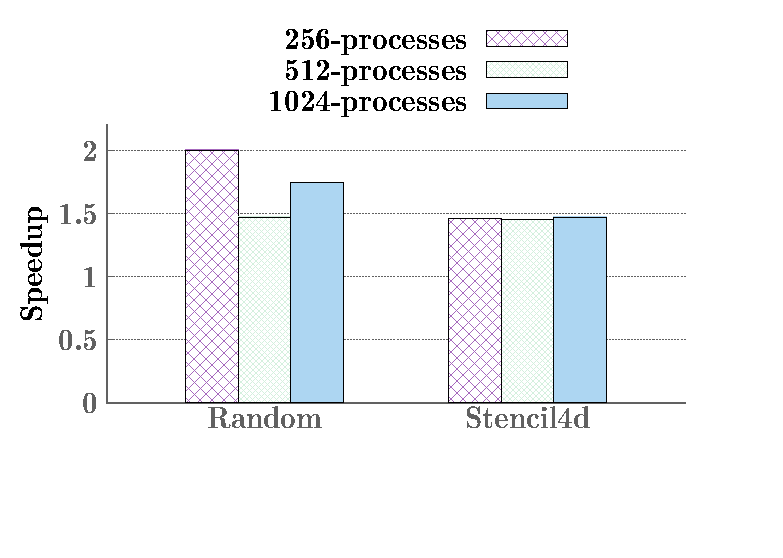
\includegraphics[width=\columnwidth]{./figs/scripts/plot_scripts/complete-info.eps}
  \caption{Speedup in latency for various techniques compared with D-mod-k for 
applications with static communication with user marked elephant flow only on fat-tree for 256, 512 and 1024 processes.}
  \label{fig:complete_info}
\end{figure}

\end{comment}


\section{Phase Identification}

HPC applications exhibit phased behavior with alternating
computation and communication phases. Since communications in different
phases do not overlap, network resources such as communication channels
allocated to communications in one phase can be reused for communications
in another phase. Hence, identifying communication phases, which is unique
in the HPC environment, allows the SDN to manage resources more effectively.

\subsection{Phase identification with user hints}

Communication phases in an HPC application can be easily identified
inside a program: there are often a section of code corresponding
for the communications in the program. Figure~\ref{code.laghos.1}
shows the code snippet for Laghos with communication phase marked. 
Here, after initiating MPI Allreduce
communications, the node performs MPI Barrier to make sure all ranks 
have the data, before initiating the computation phase where
it calculates the density.
Now, the communication pattern may be different in the two
communication phases in the given code as the comm world is calculated
at runtime. Being able to reuse network resources in different phases will
significantly improve network resource utilization. 
We propose to have an API for HPC application to give
information about phases. With the API, the user can insert a marker before
and after each communication
phase in the program to inform the network the starting and
ending of a communication phase. With the assistance from the user,
the SDN network can detect communication phases in an HPC application
without minor overheads: once all processes for an application
enter a computation phase, the application is in the computation phase and
resources for communications in the previous phase can be released; as
soon as one process enters a communication phase, the application enters
the communication phase. 

\begin{figure}[H]
\begin{lstlisting}[breaklines, language=C++, frame=single, tabsize=4, basicstyle=\ttfamily]
LagrangianHydroOperator (...){
        ...
        ParMesh *pm = H1FESpace.GetParMesh();
        MPI_Allreduce(&loc_area, &glob_area, 1, MPI_DOUBLE, MPI_SUM, pm->GetComm
());
        ...
}
\end{lstlisting}
\caption{Laghos code snippet}
\label{code.laghos.1}
\end{figure}

\begin{comment}
Communications in different phases do not happen at the same time. As such, network
resources (such as communication channels) can be allocated
independently in different phases.
Hence, accurately identifying communication phases can improve
the SDN support for HPC applications. Traditionally SDN schemes such
as the Hedera's threshold-based scheme automatically detect communication
changes when the flow statistics are collected and processed. However,
the granularity of such detection is the same as that for flow statistics
collection and processing, and network reconfiguration,
which is in the order in seconds. Such a coarse granularity is ineffective
for tightly coupled HPC applications whose phases can change in
subseconds or even submilliseconds. 
\end{comment}

%In this section we will talk about the phases of 
%HPC application and how to detect them during application runtime.

\subsection{Dynamic communication phase identification}

\begin{comment}
 Flow information used to
classify elephant flows in current phase should ignore the flow information for the flows in the
previous phase as these two set of flows  don't occur together.
In order to
determine if the network is in a communication phase, the network must be
probed at intervals smaller than the polling interval to check if data is being
sent above a certain threshold. If it is, then the network is in a
communication phase; otherwise, it is mostly in a computation phase.
If the
network transitions from a computation phase to a communication phase or vice versa during
probing, previous flow paths for elephant flows are disregarded, and the flow
informations for each flow in the current phase is considered for
prediction. 
\end{comment}

Without the hints from application, communication phases in an HPC
application can be detected by finding the computation period in the
application when very few communications are performed. 
Our dynamic communication phase identification algorithm
is shown in Figure~\ref{alg:phase_detection}. We first decide the interval
value for a minimal computation phase (e.g. 100ms). The phase detection
algorithm is executed periodically at the interval boundary to determine
whether phase is a communication phase or a computation phase depending
whether the total data communicated in the application during the phase
passes a threshold value. If a current phase is a computation phase and
the previous phase is a communication phase, network resources allocated
for the application in previous phases are released. 


\begin{algorithm}
\DontPrintSemicolon

\caption{Dynamic phase identification algorithm}
\label{alg:phase_detection}

Let Total\_data be all data sent by the application in the current interval\;
    \If{($Total\_data > Threshold$)}{
        Current phase is a communication phase\;
    }
    \Else{
      Current phase is a computation phase\;
      \If {(The previous phase is a communication phase)} {
        Release resouces allocated in previous phases
        }
    }

\end{algorithm}



\section{SDN routing}
The SDN controller has the information of the traffic in
the network. It then uses the traffic information and network information
to schedule the traffic. I call the scheduling algorithm {\em SDN-based
routing}. Clearly, SDN-based routing can be different
for different network topologies and is constrained by the underlying
network routing mechanism such as single-path routing or adaptive routing. 
In this work, I develop SDN-based routing for both full-bisection bandwidth
fat-trees and tapered fat-trees, with support for single-path as well as
adaptive routing.

I consider routing (scheduling) elephant flows that are long-lived
and bandwidth-intensive. In the discussion, I will
model the system as a directed
graph \( G = (V=S\cup N, E) \), where $N$ is the set of compute nodes,
$S$ is the set of switches, and $V$ is the set of switches ($S$) and
compute nodes ($N$), and \( E \) is the set of directed links.
The traffic demand is represented by a set of
elephant flows with each flow being denoted as a source-destination pair
$f_i = (s_i, d_i)$, where $s_i, d_i \in N$.
\[D = \{f_1=(s_1, d_1), f_2=(s_2, d_2), ..., f_n = (s_n, d_n)\}\] 

Given a traffic demand $D$, the objective of an SDN-based routing scheme is to
achieve load balancing. In the following, I will first present my SDN-based
routing for networks with single path routing and then discuss the
scheme for networks with adaptive routing.

\subsection{Single Path Routing}

For single-path routing, all packets of a flow
follow the same path. For a traffic demand
$D = \{f_1=(s_1, d_1), f_2=(s_2, d_2), ..., f_n = (s_n, d_n)\}$, 
I will denote the path for flow $f_i$ to be $p_i$, which consists of a set
of directed links. For a given routing $R$,
let $L_l$ be the set of flows that are routed through link $l$.
The load of the link $l$ is the number of flows using the link ($|S_l|$).
The load of a path $p$ is the maximum load of the loads on all links
in the path: $L_p = \max_{l \in p} {|S_l|}$. $L_p$ is referred to as the path
load. The load of the network for traffic demand $D$
is the maximum of loads among all links:
\[L_D = \max_{l\in E} {|S_l|}\]

The design objective of my SDN-based single-path routing schemes is to
minimize $L_D$ for traffic demand $D$. My first algorithm,
\textit{SDN-greedy}, is a heuristic algorithm while the second algorithm,
\textit{SDN-optimal}, is optimal for full-bisection fat trees. 

\subsubsection{SDN-greedy}

\textit{SDN-greedy} is a lightweight, single-path routing algorithm
designed to operate on both full-bisection and tapered fat-tree
topologies. As shown in Algorithm~\ref{alg:sdn_greedy}, the controller
processes each elephant flow in order. For each flow, it enumerates
all feasible paths between the source and the destination. For each
candidate path, it computes the maximum link load for the path.
The controller then selects the path with the smallest maximum link load
and assigns path to the flow.
By repeating this process for all elephant flows in the current
scheduling phase, the algorithm constructs a routing table that seeks
to keep the network-wide maximum link congestion low. This greedy
strategy effectively spreads traffic across the network. However, this
greedy algorithm may not result in the optimal scheduling for a
traffic demand, especially when the traffic is dense. 

\begin{algorithm}[H]
\DontPrintSemicolon
\caption{SDN-greedy routing}
\label{alg:sdn_greedy}
\KwInput{Elephant flows in a phase $D$}
\KwOutput{Routing table $Routing\_table$ for all flows in $D$}
\SetKwFunction{FMain}{SDN-greedy}
\SetKwProg{Fn}{Function}{:}{}
\Fn{\FMain{$D$}}{
    Initialize an empty map $Routing\_table$\;
    \ForEach{$f_i = (s_i, d_i) \in D$}{
        Get current link loads in the network\;
        Compute all possible paths for $f_i$\;
        Compute the path load for each of the possible paths based
        on the current link loads of the network\;
        Add the path with minimum path for $f_i$ to
        $Routing\_table$ for $f_i$\;
    }
    \KwRet{$Routing\_table$}\;
}
\end{algorithm}

\subsection{SDN-optimal}

While \textit{SDN-greedy} spreads the flows to paths with minimum path
loads in a greedy manner, and does not guarantee to achieve optimal $L_D$ for
a given set of elephant flows, \textit{SDN-optimal} considers the set of flows
as a whole and achieves optimal $L_D$ for full-bisection fat trees.
In the following, I will first describe SDN-optimal for full-bisection fat
trees. After that I will discuss how to extend it for tapered fat trees. 

Given traffic demand
$D = \{f_1=(s_1, d_1), f_2=(s_2, d_2), ..., f_n = (s_n, d_n)\}$, I define
$SRC_{s\in N} = \{f_i = (s_i, d_i) | s_i = s\}$ and $DST_{d\in N} =
\{f_i = (s_i, d_i) | d_i = s\}$.  $SRC_s$ is the set of flows in $D$ whose
source node is $s$ and $DST_d$ is the set of flows in $D$ whose destination
node is $d$. I define the node load for a given $D$ as 
\[NL_D = \max(\max_{s \in N} \{|SRC_s|\}, \max_{d \in N} \{|DST_d|\})\]

The node load for a traffic demand is either the maximum number of flows
coming from the same source or the maximum number of flows going to
the same destination in the traffic demand. In a fat tree topology, since
each compute node connects to one link to a switch, I have the following
theory.

{\bf Theorem 1}: For a fat-tree topology and a given traffic demand $D$,
for any single path routing scheme, $L_D \ge NL_D$.

{\em Proof:} Since each compute
node only connects one out-going link and one incoming link. Any single path
routing scheme must route the flows from a source to the out-going link that
connects to it and route the flows to a destination to the in-coming link
to the destination. Hence,
\[L_D = \max_{l\in E} {|S_l|} \ge \max_{l\ is\ a\ out-going\ link\ of\ n\in N} {|S_l|}\] and 
\[L_D = \max_{l\in E} {|S_l|} \ge \max_{l\ is\ an\ incoming\ link\ of\ n\in N} {|S_l|}.\]
Hence, 
\[L_D = \max_{l\in E} {|S_l|} \ge \max(\max_{s \in N} \{|SRC_s|\}, \max_{d \in N} \{|DST_d|\}) = NL_D.\] $\Box$

\textit{SDN-optimal} consists of two steps. Given a traffic demand $D$,
the first step is to partition $D$ into $NL_D$ permutations. In the second
step, the algorithm uses a contention free scheduling algorithm to schedule
each of the $NL_D$ permutations. Since with a contention free scheduling
algorithm, each permutation can be routed with no link contention in a
full-bisection tree. Hence, for each permutation, the maximum link load among
all links in the network
is at most 1. As a result, scheduling $NL_D$ permutations will
have a maximum link load among all links in the network of $NL_D$. In other
words, with \textit{SDN-optimal}, $L_D \le NL_D$. Hence, \textit{SDN-optimal}
is optimal for any traffic demand on a full bisection fat tree. The following
theorem summarizes this discussion. 

{\bf Theorem 2}: For a full bisection fat tree and
\textit{SDN-optimal}, for any traffic demand $D$, $L_D = NL_D$:
\textit{SDN-optimal} is optimal for the full bisection fat tree. 
$\Box$

Next, I
will give details of the two steps in the algorithm.

\paragraph{Step 1: Partitioning $D$ into $NL_D$ permutations.}
Given the traffic demand $D$, the algorithm first constructs a
bipartite graph \( G = (S, D, E) \), where \( S \) and \( D \) are
source and destination nodes in $D$, and each edge \( e \in E \) represents
a flow: if $(s, d) \in D$, then there is an edge from $s\in S$ to $d\in D$. 
This initial bipartite graph is then augmented to be a $NL_D$-regular
multi-bipartite graph by adding dummy nodes and edges. Multi-bipartite graph
allows multiple edges between two nodes. I first add dummy nodes such that
$|S|$ is the same as $|D|$. After that, I add dummy edges to make each node
in $S$ has a degree of $NL_D$ and each node in $D$ has a degree of $NL_D$.
For each node in $|S|$, if its degree is less than $NL_D$, I find a node
in $D$ whose degree is less than $NL_D$ and add a dummy edge between the
two node. This process is repeated until all nodes have $NL_D$ degree. Once
the $NL_D$-regular multi-bipartite graph is build, 
the algorithm then applies edge-coloring (via Kőnig’s Theorem)
to decompose the graph into \( NL_D \) disjoint perfect matchings ~\cite{konig1916graphen}. Each matching corresponds to a permutation
\( P_1, P_2, ..., P_{NL_D} \). The dummy edge is then removed from the
obtained permutation to yield the final permutations.
The algorithm is described in Algorithm ~\ref{alg:partition_permutations}

\begin{algorithm}[H]
\DontPrintSemicolon
\caption{Flow partitioning into disjoint permutations}
\label{alg:partition_permutations}

\KwInput{Flow set $D$}
\KwOutput{$NL_D$ disjoint permutations $P_1, ..., P_{NL_D}$}

Construct bipartite graph $G = (S, D, E)$ from flows in $F$\;

Pad $G$ with dummy nodes and edges to make it $NL_D$-regular multi-bipartite
graph\;

Apply edge-coloring to obtain $NL_D$ disjoint matchings $P_1, ..., P_{NL_D}$\;

Remove dummy flows from each $P_i$\;

\KwRet{$P_1, ..., P_k$}
\end{algorithm}

\paragraph{Step 2: Contention-free scheduling for each permutation}  

Finding a contention-free schedule for a permutation on a full-bisection
fat-tree topology has been investigated for more than two decades, and a
number of efficient algorithms are now available\,%
\cite{Paull1962,Rodriguez2009,Zahavi2010,Prisacari2013}.  In this work, I
represent the permutation with a connection
matrix,\cite{Paull1962} and apply the coloured-matrix algorithm of
Rodríguez \emph{et al.}\,\cite{Rodriguez2009}, thereby ensuring that each
permutation is routed without link contention.

\subsubsection{SDN-optimal for Tapered Fat-trees}

In a tapered fat-tree, bandwidth reduction occurs at higher layers,
such as the aggregate to core level has less links than leaf to aggregate
level. This architectural tapering leads to insufficient link capacity
when routing permutation traffic, where the number of flows often
exceeds the number of available links at higher levels.
As a result, \textit{SDN-optimal} does not work on tapered fat-trees
since achieving a contention-free assignment for all flows within a
single permutation becomes infeasible.

To overcome this limitation, the SDN-optimal routing strategy
partitions the full permutation into multiple sub-permutations.
Each sub-permutation is constructed such that the number of flows
passing through each layer of the network matches the number of
available links at that layer. This ensures that within each
sub-permutation, contention-free routing is still possible using
the techniques previously employed.

My goal is to make sure that I create sub-permutations by
selecting flows in such a way that the links in between each
fat-tree layers have no contention and has the maximum utilization. 
To construct these sub-permutations, the algorithm first selects
flows that traverse the core layer, typically inter-pod flows that consume both leaf-to-aggregate and aggregate-to-core links. It continues selecting such flows until all available core-level links are utilized. At this point, adding more inter-pod flows would introduce contention. The algorithm then fills the remaining capacity at the aggregation layer by selecting intra-pod flows, which consume only leaf-to-aggregate and aggregate-to-leaf links. The result is a sub-permutation that fully utilizes available link resources without exceeding capacity at any layer. This allows Hall’s Marriage Theorem \cite{cameron2025hall} \cite{hall1987representatives} to be applied to guarantee a conflict-free routing for each sub-permutation.

\begin{algorithm}[H]
\caption{Sub-permutation construction}
\label{alg:sub_permutation}
\KwIn{
    $F_{\text{core}}$: Set of flows that traverse the core switch\\
    $F_{\text{agg}}$: Set of flows that only traverse the aggregate switch\\
    $c$: Number of available core-to-aggregate links per sub-permutation\\
    $a$: Number of available aggregate-to-leaf links per sub-permutation
}
\KwOut{
    $P_{\text{list}}$: list of sub-permutations
}

$P_{\text{list}} \gets \emptyset$\;

\While{$F_{\text{core}} \neq \emptyset$ \textbf{or} $F_{\text{agg}} \neq \emptyset$}{
    $P \gets \emptyset$\;
    $core\_links \gets c$\;
    $agg\_links \gets a$\;

    \tcp{Stage 1: Add core-level flows}
    \ForEach{$f \in F_{\text{core}}$}{
        Add $f$ to $P$\;
        $core\_links \gets core\_links - 1$\;
        Remove $f$ from $F_{\text{core}}$\;
        \If{$core\_links == 0$ \textbf{or} $F_{\text{core}} == \emptyset$}{
            \textbf{break}
        }
    }

    \tcp{Stage 2: Add aggregate-level flows}
    \ForEach{$f \in F_{\text{agg}}$}{
        Add $f$ to $P$\;
        $agg\_links \gets agg\_links - 1$\;
        Remove $f$ from $F_{\text{agg}}$\;
        \If{$agg\_links == 0$ \textbf{or} $F_{\text{agg}} == \emptyset$}{
            \textbf{break}
        }
    }

    Append $P$ to $P_{\text{list}}$\;
}

\Return $P_{\text{list}}$\;
\end{algorithm}

\subsection{Adaptive Routing}

Adaptive routing enables traffic to be split across multiple paths adaptively
based on the network condition, improving bandwidth utilization and often
reducing congestion. This is a very effective routing scheme for fat-tree.
However, in many scenarios where flow paths overlap significantly, causing
contention. On the other hand, for a full bisection bandwidth fat-tree, any
permutation traffic including the shift traffic pattern can be scheduled
without contention using single-path routing. Hence, for such traffic pattern,
using single path routing can achieve higher performance than
adaptive routing. Based on this observation, I propose \textit{SDN-adaptive}
that adapt between these two strategies: if the traffic demand $D$ is
less than a permutation, use SDN-optimal; otherwise, use the underlying
adaptive routing.

%I propose \textit{SDN-adaptive} routing for the multipath routing.
%\subsubsection{SDN-adaptive}
%The key idea behind SDN-adaptive is to first gather runtime information about the application’s traffic characteristics. During an initial profiling phase, SDN-adaptive collects communication performance data by running one iteration using adaptive multipath routing. This information is then sent to the SDN controller, which uses it decide the routing.
%The process begins by executing one iteration of the application using adaptive multipath routing. The SDN controller records the communication time from this iteration as a reference. Then, the full simulation is restarted using SDN-optimal routing. After completing the first iteration of this SDN-optimal run, the controller compares the current communication time with the previously recorded time from the adaptive run.
%
%If SDN-optimal demonstrates better performance (i.e., lower communication time), it is retained for the rest of the simulation. If, however, SDN-optimal is slower than adaptive, this indicates that multipath routing is more effective for the application's communication pattern. In that case, the controller immediately switches to adaptive routing for the remainder of the simulation.
%
%This design allows the routing policy to be tuned to the observed behavior of the application, ensuring better adaptability across diverse workloads. The algorithm is described in algorithm ~\ref{alg:sdn_adaptive_api}

%\begin{algorithm}[H]
%\DontPrintSemicolon
%\caption{SDN-adaptive algorithm}
%\label{alg:sdn_adaptive_api}
%
%\KwInput{%
%  Application $A$; \\
%  Topology $G$; \\
%  Routing schemes: SDN-optimal and Adaptive
%}
%\KwOutput{%
%  Final routing strategy and flow configuration
%}
%
%Run one iteration of $A$ using Adaptive routing\;
%Record $\mathrm{commTime}_{\text{Adaptive}}$\;
%
%Start full simulation of $A$ using SDN-optimal routing\;
%After first iteration, record $\mathrm{commTime}_{\text{SDN-optimal}}$\;
%
%\If{$\mathrm{commTime}_{\text{SDN-optimal}} < \mathrm{commTime}_{\text{Adaptive}}$}{
%  Continue simulation with SDN-optimal routing\;
%}
%\Else{
%  Switch to Adaptive routing for remainder of simulation\;
%}
%\end{algorithm}


\section{Experimental Setup}
I perform extensive experiments using the TraceR-CODES simulator~\cite{jain2016evaluating,mubarak2016enabling}, which I have extended to support the study of the SDN techniques discussed in this work. TraceR-CODES is a software tool suite used for performance analysis of parallel and distributed applications, and it is specifically designed to simulate large-scale scientific applications running on high-performance computing systems.

To support my experiments, I have integrated the trained DNN model into the simulator using Google TensorFlow's C APIs. To ensure compatibility with the TensorFlow libraries, I carefully selected the MPI and GNU compiler standards. In particular, I utilized MVAPICH 2 as the MPI implementation and adopted C++14 from GNU version 9.0.1 as the compiler standard.

By leveraging real-time network statistics, my DNN model dynamically predicts network flows during the simulation runtime. This capability not only enhances prediction accuracy but also enables real-time data processing, making the model both robust and efficient.

In addition to evaluating SDN-based routing, I also investigate the impact of hardware design characteristics on performance using the Fat-tree connection topology. The Fat-tree topology is a well-established interconnect architecture commonly employed in HPC systems and data centers. I conduct simulations on two distinct Fat-tree configurations: a 1024-node full-bisection Fat-tree and a 1536-node tapered Fat-tree with a 3:1 oversubscription ratio. In both configurations, each switch is equipped with 32 ports, and each leaf switch connects to 16 compute nodes. Importantly, all 32 ports of the core and aggregate switches are fully utilized, connecting exclusively to other switches to preserve the hierarchical structure of the topology.

In this study, I explore three types of SDN routing mechanisms:

SDN-greedy, which allocates paths by minimizing congestion in real time using simple heuristics;

SDN-optimal, which computes globally least-congested paths by evaluating all possible routes;

SDN-adaptive, which dynamically adjusts routing decisions based on the current traffic patterns and flow types.

For flow classification, I employ three distinct strategies:

Threshold-based, where flows are classified as elephant or mice based on a predefined data volume threshold;

DNN-based, where a trained deep neural network identifies flow types based on extracted runtime features;

User input, where the application provides direct hints to classify communication flows.

Each of these methods is described in detail in earlier sections of this work. Below is the table outlining the network configuration parameters used in the simulation.

\begin{table}[h]
\centering
\caption{Network parameters for simulation of SHS}
\label{tab:params}
\vspace{1em}
\begin{tabular}{ll}
\toprule
Parameter & Value \\
\midrule
Packet Size     & 8192 Bytes \\
Switch Radix    & 32 \\
Link Bandwidth  & 11.9 GB/s \\
Eager Limit     & 64000 Bytes \\
NIC Scheduler   & Round-robin \\
\bottomrule
\end{tabular}
\end{table}



To mitigate the impact of various types of delay on our data, specifically in 
the communication aspect of the experiment, we have configured the router 
delay, network interface controller (NIC) delay, software delay, and remote 
direct memory access (RDMA) delay to zero. This setup allows us to eliminate 
any extraneous delay factors and isolate the effects of the communication 
process on our data analysis.


\section{Application and Workloads}
Eight representative applications are used in the study:
\texttt{Random-Permutation}, \texttt{Shift}, \texttt{Stencil3d}, \texttt{Stencil4d}, \texttt{Milc}, and \texttt{Nekbone}, \texttt{Random-Permutation-Mixed},
and \texttt{Stencil-Mixed}. All of the applications except \texttt{Random-Permutation-Mixed} and \texttt{Stencil-Mixed} including 
their computation and communication characteristics have been described
in detail in Chapter 2.

\begin{itemize}
\item \textbf{Random-Permutation-Mixed}: This pattern alternates between two distinct random-permutation communication phases, separated by a computation phase. Each communication phase uses a different source-destination mapping, introducing dynamic changes in the communication structure.

\item \textbf{Stencil-Mixed}: This application combines a \texttt{Stencil3d} phase followed by a \texttt{Stencil4d} phase, with an intermediate computation phase. The transition between patterns allows evaluation of the routing system’s responsiveness to changes in spatial communication demands.
\end{itemize}

All of these applications are communication-intensive, but 
they exhibit diverse communication behaviors ranging from synthetic
near-neighbor patterns to production-level scientific codes
and serve as appropriate test cases to assess how well SDN techniques
manage different types of network traffic.

To ensure accurate analysis of communication transitions, I enforce
explicit synchronization barriers between phases. This guarantees
that each communication phase is fully completed before the next begins,
preventing overlap and allowing isolated assessment of routing behavior across phases.

\section{Performance Study}
The result of various SDN techniques which are used in HPC is presented here

\subsection{Evaluation of flow classification techniques}

In this section, we compare the impact of different flow identification techniques on the SDN algorithm for various applications under full bisection fat-tree and 3-to-1 tapered fat-tree configurations. The evaluation includes performance metrics across application communication time for different applications. To evaluate the flow detection technique, we kept the routing fixed as SDN‑optimal and used communication‑computation phase detection, while varying the flow detection methods.

\subsubsection{Performance Under Full Fat-Tree}
\begin{figure}[h]
  \centering
  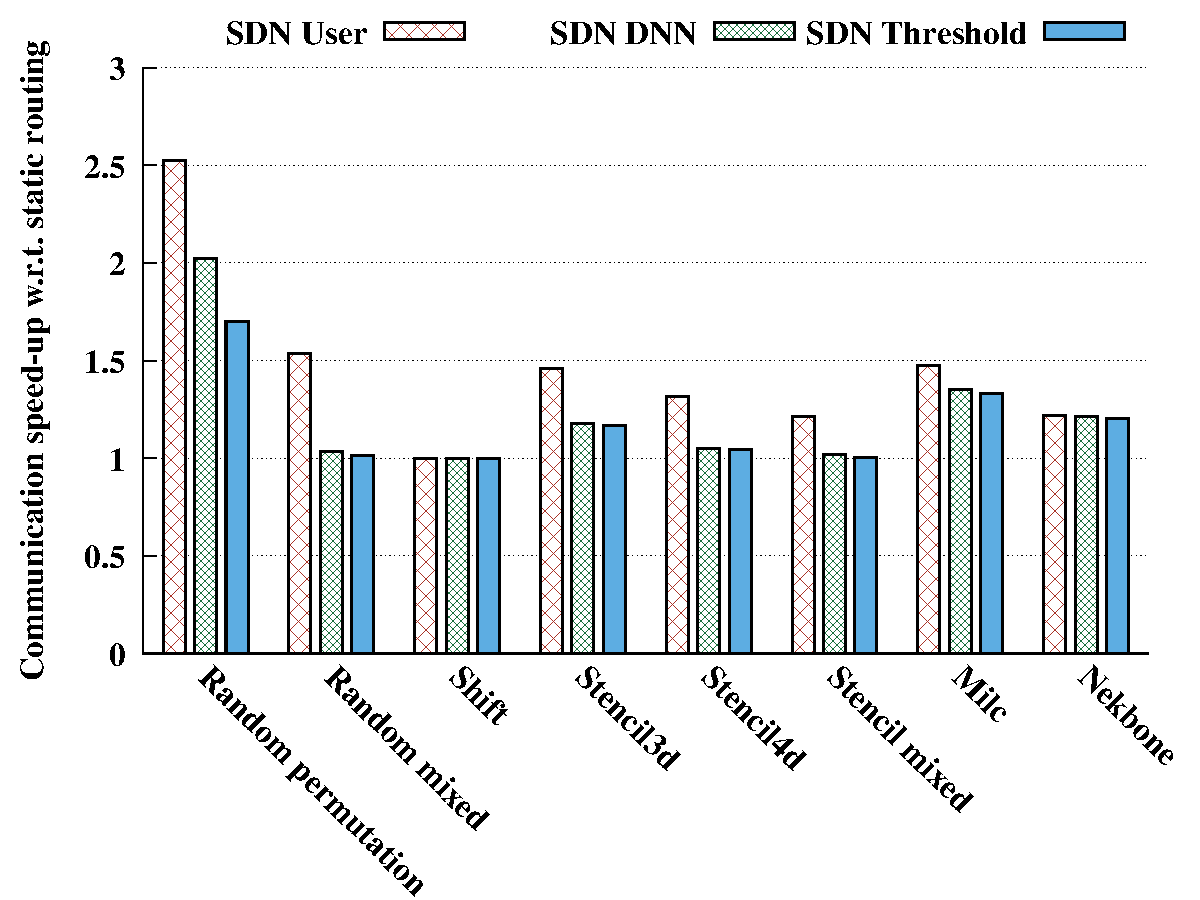
\includegraphics[width=\columnwidth]{./figs_4/full_fat_flow_detection.pdf}
  \caption{Comparison of flow detection in full bisection fat-tree of 1024 nodes}
  \label{fig:fld_full}
\end{figure}

The Figure ~\ref{fig:fld_full} compares communication speedup achieved by three flow detection techniques, SDN User, SDN DNN, and SDN Threshold across various applications, including Random-Permutation, Random-mixed Shift, Stencil3D, Stencil4D, Stencil-mixed, Milc, and Nekbone. These applications represent diverse traffic patterns, ranging from simple to highly complex workloads, making them ideal benchmarks for evaluating network performance.  A higher bar (speedup) signifies better efficiency and lower communication time relative to the baseline. The user flow identification technique performs best due to early flow identification, enabling prompt traffic management. DNN detection ranks second, limited by a 0.3-millisecond delay. Threshold detection performs worst due to delayed flow recognition. Importantly, all three techniques perform better than the widely used single-path static routing, demonstrating the effectiveness of dynamic flow detection in improving communication efficiency within SDN frameworks. User detection consistently leads across all applications. DNN detection shows reasonable gains despite initial delay. Threshold detection offers minimal improvement. These results highlight the importance of incorporating flow detection mechanisms to enhance SDN routing performance beyond conventional static routing methods like D-mod-K, also, the DNN model does a faster flow classification compared to threshold based model without losing in performance.


\begin{comment}
\begin{figure*}[t]
  \centering
  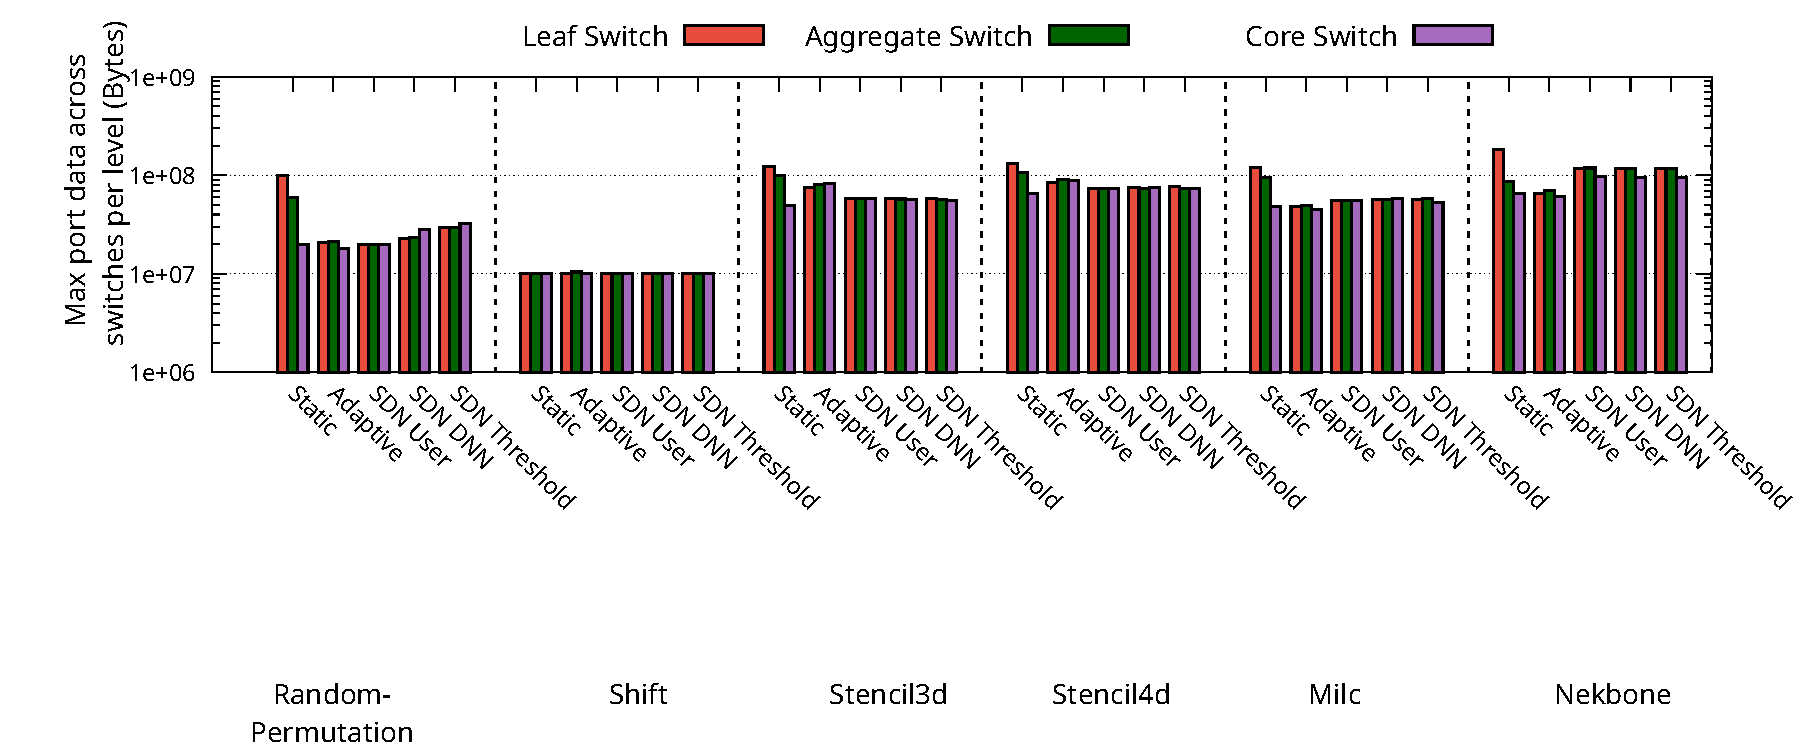
\includegraphics[width=\textwidth]{./figs_4/combined_max_load_plot_full.pdf}
  \caption{Max data sent through a port in a switch level for all switches in full bisection fat-tree of 1024 nodes}
  \label{fig:ld_full}
\end{figure*}



The Figure ~\ref{fig:ld_full} shows maximum outgoing data (Bytes) through ports across six application sections: Random-Permutation, Shift, Stencil3D, Stencil4D, MILC, and Nekbone. Each section contains bars representing three configurations:
Green represents the maximum load at the leaf switches, Blue indicates the maximum load at the aggregate switches, and Red signifies the maximum load at the core switches. Observations reveal that the Random-Permutation application shows the highest load at the leaf switch under the Static configuration. Similarly, Stencil3D and Stencil4D exhibit high loads at both leaf and aggregate switches in Static and Adaptive configurations. Nekbone records the highest outgoing data, particularly at the leaf switch under the Static configuration. When comparing SDN loads, they are consistently lower than those in Static configurations and remain lower than Adaptive configurations when communication density is moderate, as observed in applications like Random-Permutation, Shift, Stencil3D, and Stencil4D. SDN effectively distributes loads across ports, resulting in a positive speedup over static routing.
\end{comment}

\subsubsection{Performance Under Tapered Fat-Tree}
\begin{figure}[h]
  \centering
  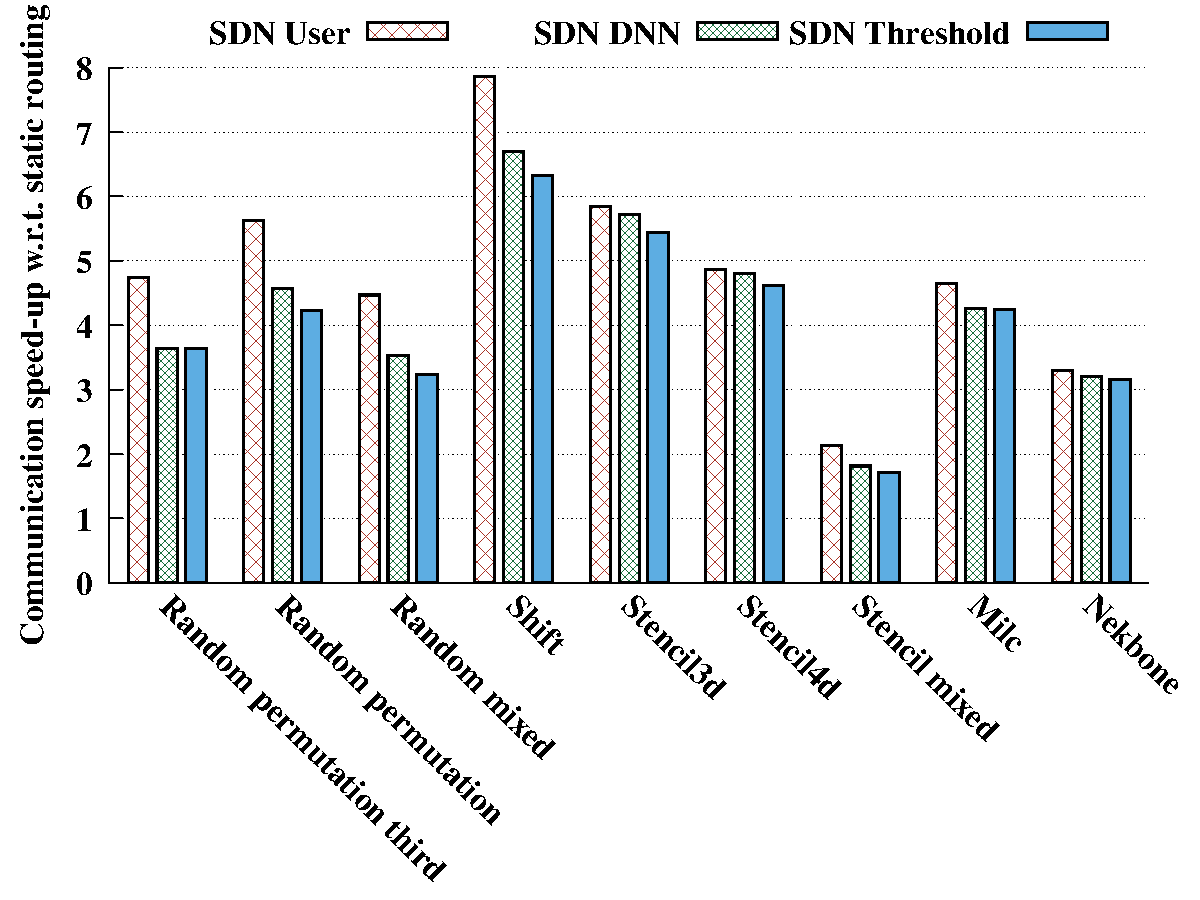
\includegraphics[width=\columnwidth]{./figs_4/taper_fat_flow_detection.pdf}
  \caption{Comparison of flow detection in 3 to 1 taper fat-tree of 1536 nodes}
  \label{fig:fld_taper}
\end{figure}

The Figure ~\ref{fig:fld_taper} illustrates the communication speedup achieved by different flow detection techniques (SDN User, SDN DNN, and SDN Threshold) under a 3-to-1 taper fat-tree topology with 1536 nodes and a 3:1 tapering ratio. This topology emphasizes the impact of reduced bandwidth at higher levels of the Fat-Tree structure.


In a tapered fat-tree topology, even a random-permutation pattern represents a relatively dense communication workload. To better demonstrate the effectiveness of our routing mechanism in balancing traffic, we introduced Random-Permutation-Third by removing two-thirds of the communication from a random-permutation of 1536 nodes, retaining only eight out of the 24 communication flows passing through a leaf router. Our evaluation revealed that SDN User consistently achieved the highest speedup, exceeding 6x, highlighting the benefits of early user-provided flow identification that enables optimal traffic balancing from the start. In contrast, SDN DNN and SDN Threshold exhibited moderate speedups of approximately 1.5x and 1.2x, respectively, due to delayed flow detection. Similar trends were observed in the Shift application, where SDN User maintained its superior performance, while SDN DNN and SDN Threshold provided moderate improvements over static routing. In compute-heavy applications such as Milc and Nekbone, the performance gap between techniques narrowed, though SDN User remained the top performer. The results suggest that compute-heavy traffic benefits from steady-state optimizations, though early flow detection consistently outperformed or matched the threshold-based approach. These findings underscore the critical role of early flow detection in achieving optimal traffic balancing, particularly in tapered Fat-Tree topologies with constrained bandwidth, as reflected by higher speedup values relative to baseline D-mod-K routing.


\begin{comment}
\begin{figure*}[t]
  \centering
  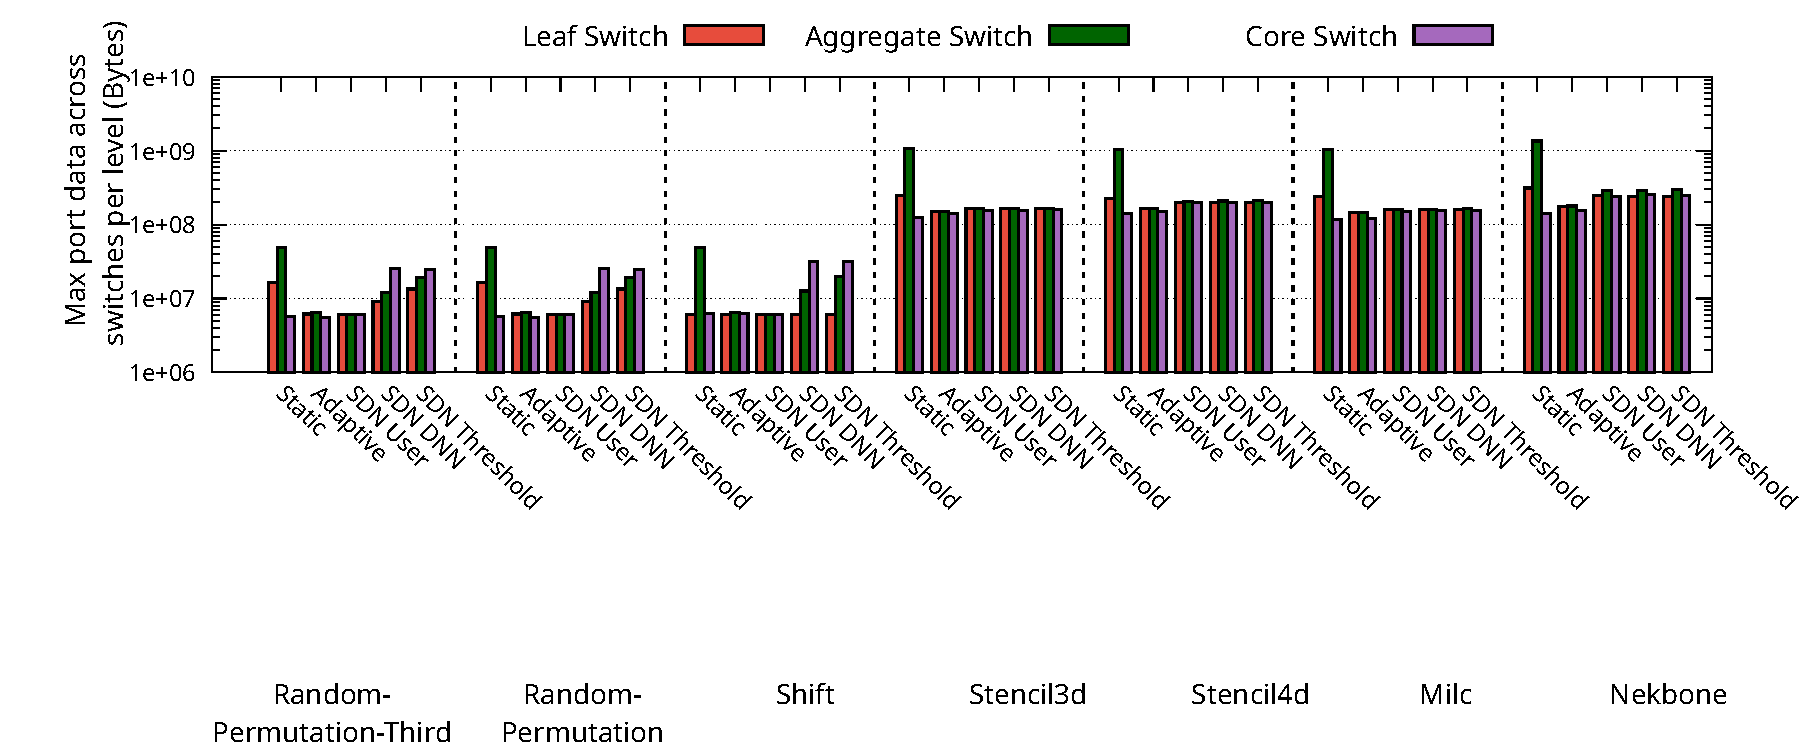
\includegraphics[width=\textwidth]{./figs_4/combined_max_load_plot_taper.pdf}
  \caption{Max data sent through a port in a switch level for all switches in 3-to-1 taper fat-tree of 1536 nodes}
  \label{fig:ld_taper}
\end{figure*}


In tapered, the aggregate switch ports have a lot of load, and in all cases, SDN with all various flow identification techniques have always drtibuted this load across the the other switch ports. SDN performance in load distribution is almost same as adaptive and in cases for Shift and Random-Permutation-Third it is doing a slightly better job than adaptive.



%
%
%
%
%
%          next Sub Section 2 of results
%
%
%
%
%

\end{comment}

\subsection{Evaluation of Phase Identification}
This section evaluates the effectiveness of phase identification, across varioous applications under full bisection fat-tree and 3-to-1 tapered fat-tree configurations. To evaluate the communication‑computation phase identification technique, we kept the routing fixed as SDN‑optimal and used the SDN user flow detection method, while varying the phase identification methods.

\subsubsection{Performance Under Full Fat-Tree}


\begin{figure}[h]
  \centering
  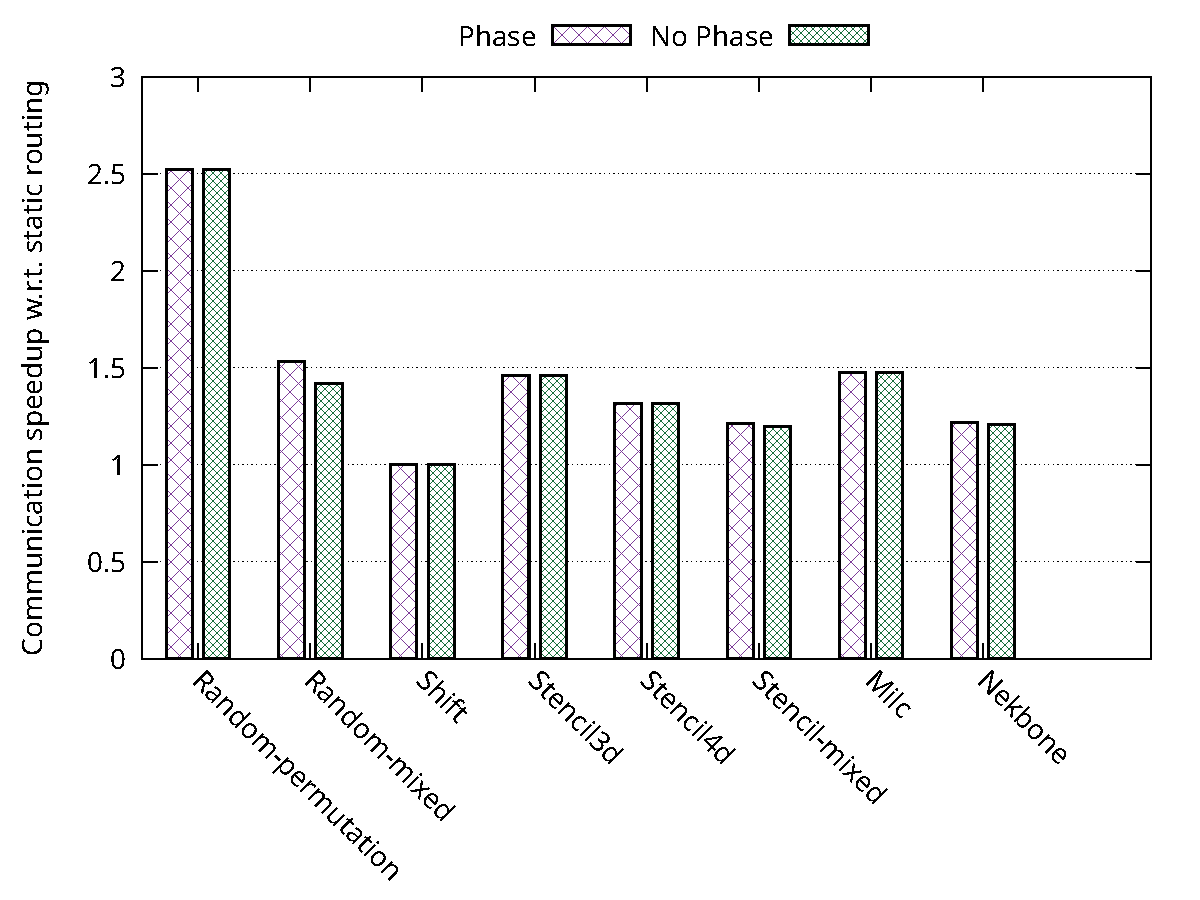
\includegraphics[width=\columnwidth]{./figs_4/phase_full.pdf}
  \caption{Comparison of phase identification in full bisection fat-tree of 1024 nodes}
  \label{fig:phase_full}
\end{figure}
The Figure~\ref{fig:phase_full} shows phase identification results for full Fat-tree, where the x-axis represents different workloads, including Random-permutation, Random-mixed, Shift, Stencil3d, Stencil4d, Stencil-mixed, Milc, and Nekbone, while the y-axis quantifies the relative speedup. 
In Full Fat-Tree routing, phase-based optimization leverages threshold-based flow classification and SDN routing to improve communication efficiency. The analysis of communication speedup reveals notable improvements in random-mixed, stencil-mixed, and nekbone, with random-mixed achieving a 7.98\% increase in performance. The phase identification mechanism efficiently distinguishes between different communication phases. When a phase transition occurs, it promptly loads the corresponding routing table, ensuring seamless adaptation to dynamic communication patterns.

The evaluation time for each phase is one-tenth of a polling phase, during which the phase identifier continuously monitors network flows to detect transitions between computation and communication phases. Upon detecting a phase change, it swiftly loads the appropriate routing table to optimize data flow. In random-mixed, stencil-mixed, and nekbone, frequent transitions between computation and communication phases trigger rapid routing table updates, leading to measurable performance improvements in these applications.


\subsubsection{Performance Under Tapered Fat-Tree}
\begin{figure}[h]
  \centering
  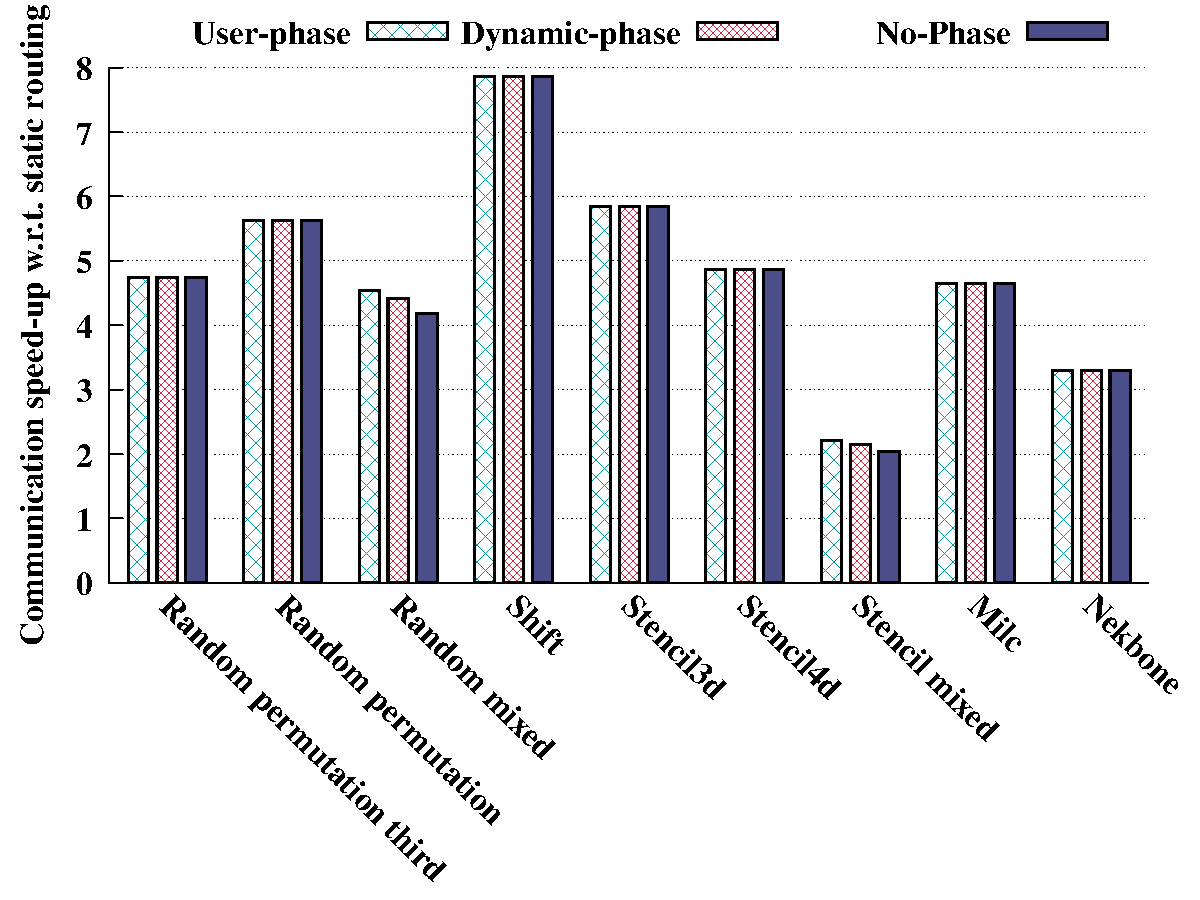
\includegraphics[width=\columnwidth]{./figs_4/phase_taper.pdf}
  \caption{Comparison of phase identification in full bisection fat-tree of 1536 nodes}
  \label{fig:phase_taper}
\end{figure}
The Figure~\ref{fig:phase_taper} shows phase identification results for full Fat-tree,
In Tapered Fat-Tree routing, phase-based optimization dynamically adjusts traffic injection rates using threshold-based flow classification and SDN routing to further enhance communication efficiency. The analysis of communication speedup shows notable improvements in random-mixed, stencil-mixed, and nekbone, with random-mixed achieving an 11.13\% increase in performance, surpassing the gains observed in Full Fat-Tree routing. The phase identification mechanism efficiently detects phase transitions and dynamically manages traffic flow to reduce network congestion

\subsection{Evaluation of SDN-based Routing}
This section evaluates the effectiveness of SDN-based routing approaches across various applications under full bisection fat-tree and 3-to-1 tapered fat-tree configurations of user identification of flows. We analyze performance in terms of communication times.To evaluate the various SDN routing techniques, we kept the communication‑computation phase identification fixed and used the SDN user flow detection method, while varying the SDN routing methods.

\subsubsection{Performance Under Full Fat-Tree}
The Figure ~\ref{fig:routing_full} illustrates the communication speedup achieved by three routing techniques—Adaptive, SDN User, and SDN-Adaptive across various applications under a full fat-tree topology. The y-axis represents the speedup relative to static D-mod-K routing, where higher bars indicate better performance.


\begin{figure}[h]
  \centering
  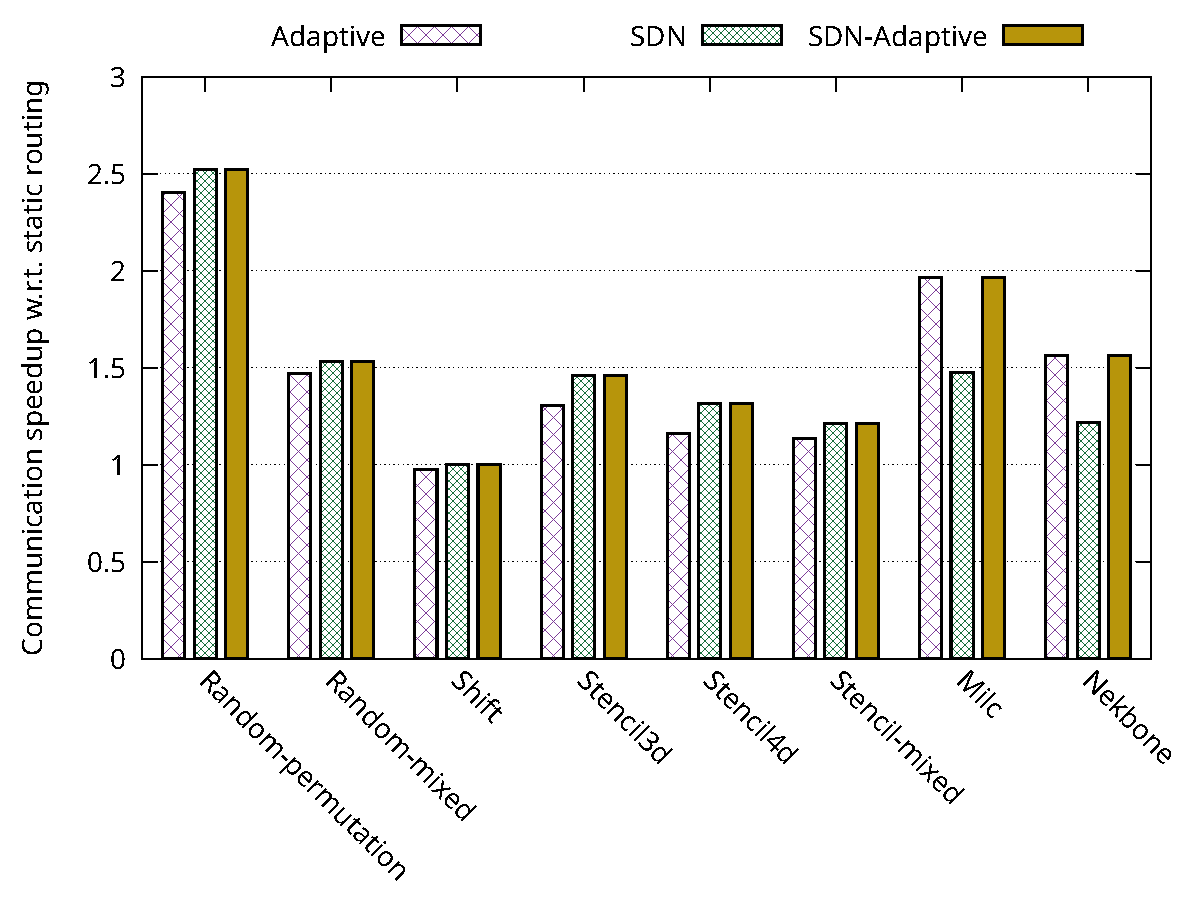
\includegraphics[width=\columnwidth]{./figs_4/routing_full.pdf}
  \caption{Comparison of routing techniques in full fat-tree of 1024 nodes}
  \label{fig:routing_full}
\end{figure}
Single-path SDN routing consistently outperforms single-path DmodK routing across all scenarios.

While SDN routing generally performs better than Adaptive routing, the multipath nature of Adaptive routing allows it to balance the load more effectively when communication becomes dense. At this point, SDN-Adaptive, a hybrid approach combining SDN and Adaptive strategies, performs similarly to Adaptive routing at high communication density application and similar to SDN then the communication density is low, leveraging its flexibility to adapt based on the application's requirements.

\begin{comment}
\begin{figure}[t]
  \centering
  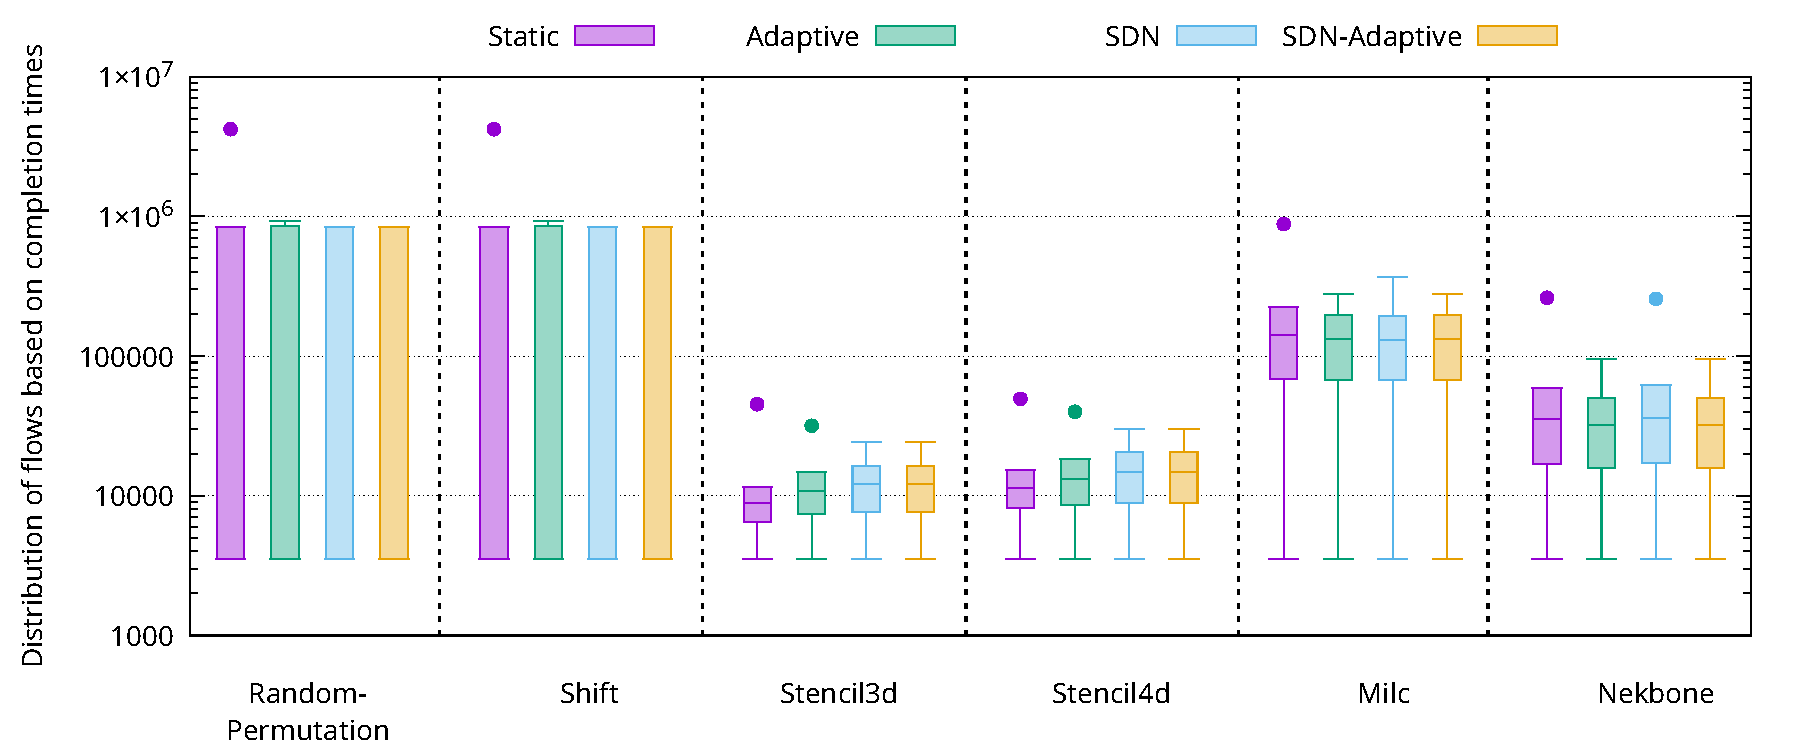
\includegraphics[width=\columnwidth]{./figs_4/two_column_multiplot_boxplots_full.pdf}
  \caption{Distribution of flow completion times in full fat-tree of 1024 nodes}
  \label{fig:flow_dist_full}
\end{figure}


The Figure ~\ref{fig:flow_dist_full} show the distribution of distribution of flows based on flow completion times. 
\end{comment}

SDN even being a single path routing is kind of making sure that flows are completing together and there is no stragglers left behind. 


\subsubsection{Performance Under Tapered Fat-Tree}



\begin{figure}[h]
  \centering
  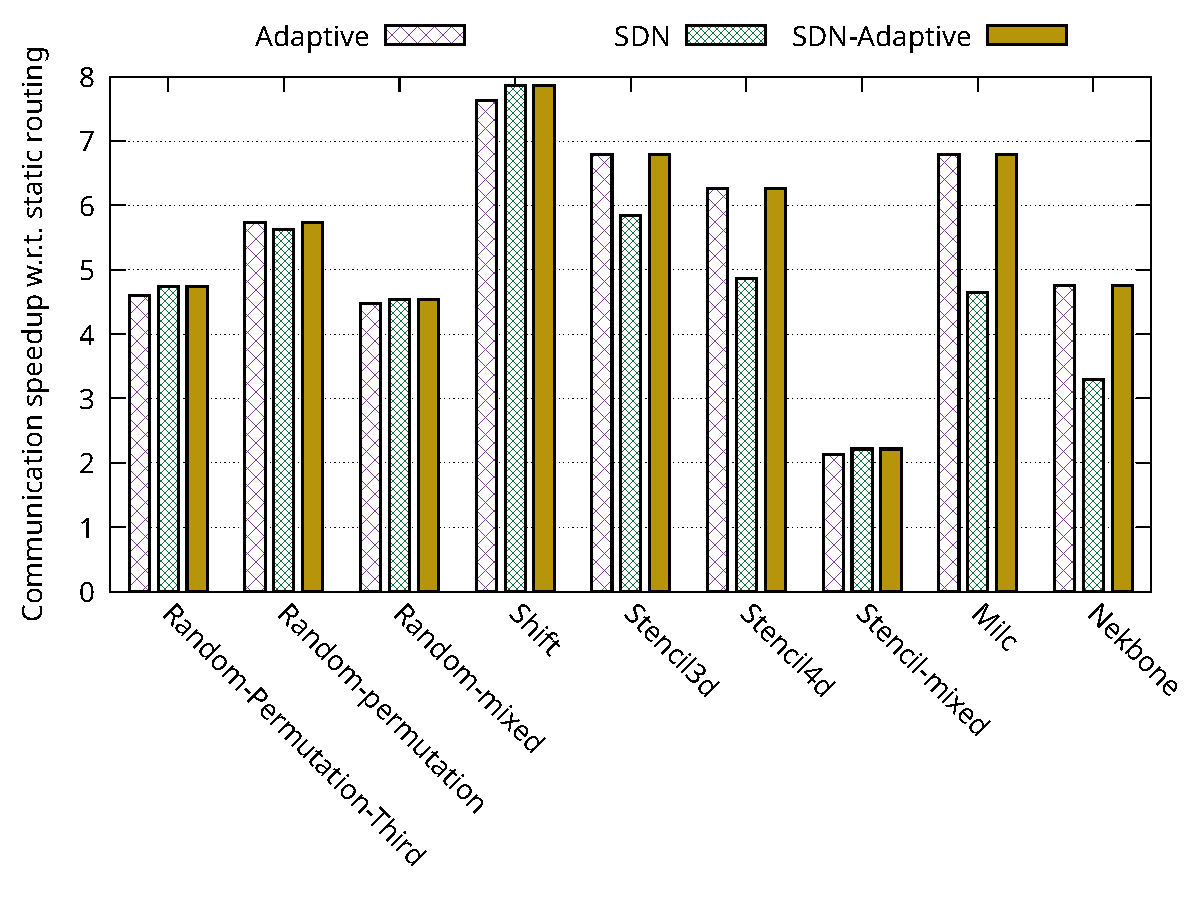
\includegraphics[width=\columnwidth]{./figs_4/routing_taper.pdf}
  \caption{Comparison of routing techniques in 3 to 1 taper fat-tree of 1536 nodes}
  \label{fig:routing_taper}
\end{figure}


The Figure ~\ref{fig:routing_taper} presents a comparison of routing techniques (Adaptive, SDN User, and SDN-Adaptive Use) across three applications (Random-Permutation, Shift, and Milc) under a Tapered Fat-Tree topology. The y-axis represents the communication speedup relative to DmodK routing, where higher bars indicate better performance. In a Tapered Fat-Tree topology, applications typically experience dense traffic patterns due to limited bandwidth at higher levels caused by tapering. Adaptive routing demonstrates strong performance in balancing network load, especially under traffic-heavy scenarios. However, in Random-Permutation-Third, where traffic is reduced, our evaluation clearly shows that SDN-based routing outperforms adaptive routing. In Shift traffic patterns, where traffic predictability is higher, Adaptive routing effectively balances the load better than static routing, though SDN-based routing still makes slightly better decisions due to its global network awareness. SDN-Adaptive routing leverages the strengths of both Adaptive and SDN-based routing by dynamically adapting to application-specific traffic patterns, selecting the most suitable approach for optimal performance. 

\begin{comment}
\begin{figure}[t]
  \centering
  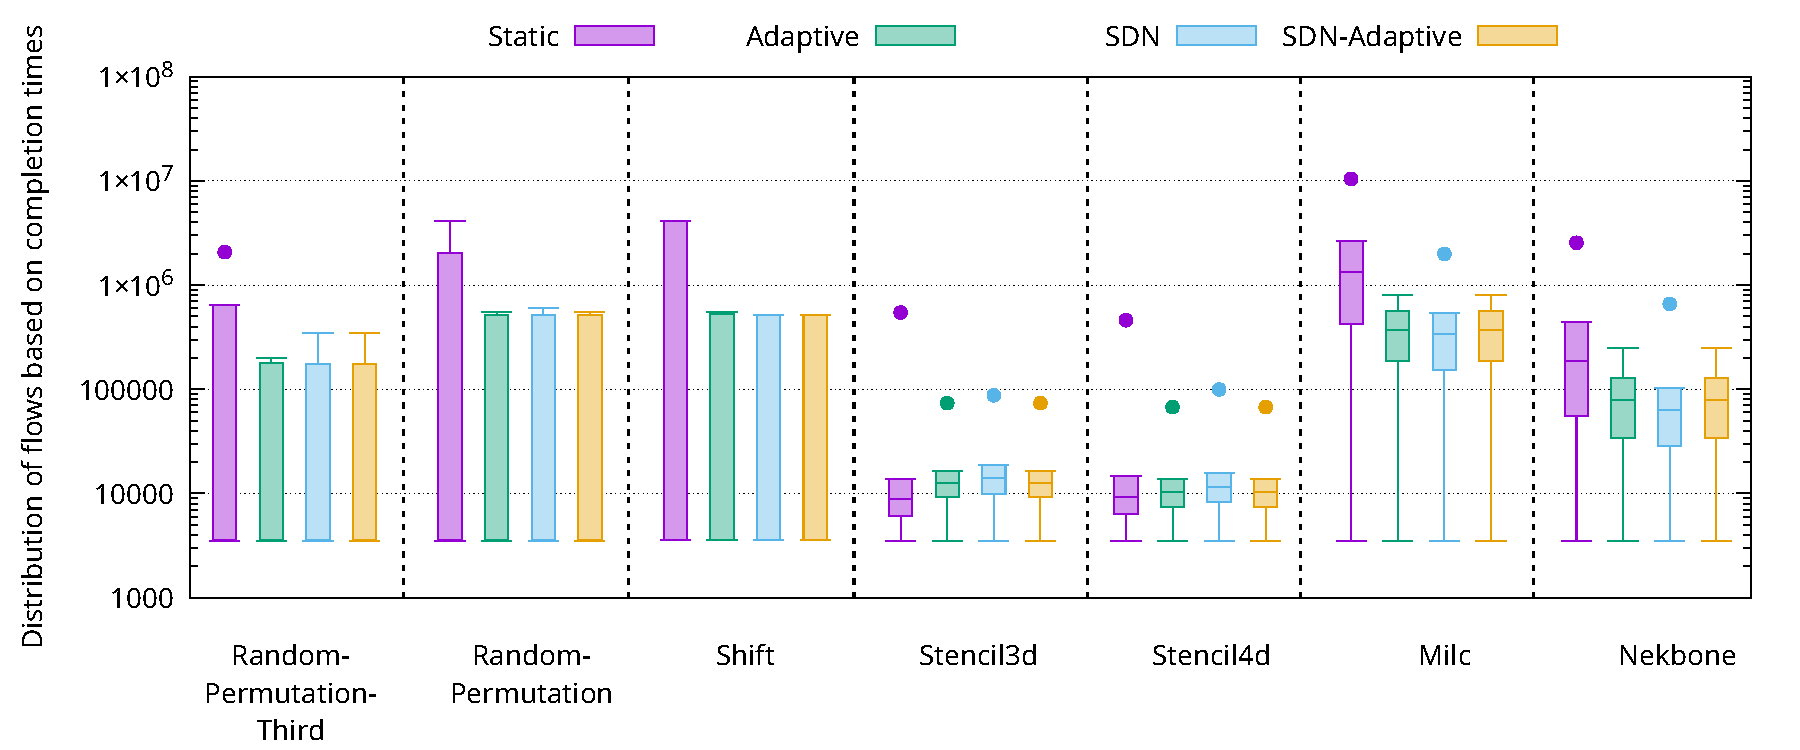
\includegraphics[width=\columnwidth]{./figs_4/two_column_multiplot_boxplots_taper.pdf}
  \caption{Distribution of flow completion times in 3-to-1 taper fat-tree of 1536 nodes}
  \label{fig:flow_dist_taper}
\end{figure}


The Figure ~\ref{fig:flow_dist_full} illustrates the flow completion time distribution. Despite utilizing a single-path routing approach, SDN effectively ensures that flows complete within a similar timeframe, minimizing the presence of stragglers. This highlights the capability of SDN to maintain consistent flow completion, reducing delays and enhancing overall network performance.
\end{comment}

\section{Summary}
This chapter investigated the adaptation of SDN techniques to HPC systems whose
communication patterns are distinguished by repetitive compute-and-communicate
phases. Central to the study was an extensive TraceR-CODES simulation that
examined three interlocking SDN control-plane mechanisms—flow identification,
phase identification, and flow scheduling—across two representative
interconnects: a 1024-node full-bisection fat-tree and a 1536-node 3-to-1
tapered fat-tree. The study first demonstrated that early, user-based flow
classification delivers the greatest performance gains, while a
deep-neural-network classifier offers an accurate, low-latency alternative and a
threshold scheme provides a baseline. It then revealed that distinguishing
computation from communication phases allows the network to quickly release
resources, reducing worst-link congestion by in both full
fat-trees and tapered counterparts. Finally, the evaluation of
three SDN-based routing algorithms, SDN-greedy, SDN-optimal, and a hybrid
SDN-adaptive strategy—showed that SDN-optimal minimizes maximal link load and
outperforms conventional adaptive routing when traffic density is low, whereas
SDN-adaptive dynamically shifts between optimal and adaptive behavior, achieving
up to six to seven fold reductions in communication time under
bandwidth-constrained conditions, specifically in tapered fat-trees.
Collectively, these findings advance a holistic perspective in which rapid flow
classification, phase-aware resource reclamation, and traffic-aware routing are
orchestrated to elevate network efficiency. Because the proposed techniques
depend only on flow semantics and relative link abundance, they extend naturally
to the irregular, tapered fat-tree variants prevalent in production clusters,
thereby offering a practicable pathway toward more agile and capable SDN-based
HPC system.
Drawing on the insights established in this groundwork, the following chapter identifies 
the hardware parameters that best support HPC applications in modern HPC systems.

